\documentclass[utf8]{beamer}

% This file is a solution template for:

% - Talk at a conference/colloquium.
% - Talk length is about 20min.
% - Style is ornate.

\mode<presentation>
{
  \usetheme{Warsaw}
  % or ...

  \setbeamercovered{transparent}
  % or whatever (possibly just delete it)
}


\usepackage[english]{babel}

\usepackage[utf8]{inputenc}
% or whatever

\usepackage{times}
\usepackage[T1]{fontenc}
% Or whatever. Note that the encoding and the font should match. If T1
% does not look nice, try deleting the line with the fontenc.


\title{A flexible Prolog interpreter in Python}

\author{Carl Friedrich Bolz}
% - Give the names in the same order as the appear in the paper.
% - Use the \inst{?} command only if the authors have different
%   affiliation.

\institute[Heinrich-Heine-Universität Düsseldorf]
{
  Institut für Informatik\\
  Heinrich-Heine-Universität Düsseldorf
}

\date{24. Workshop der GI-Fachgruppe Programmiersprachen und Rechenkonzepte, 4. Mai 2007}
% - Either use conference name or its abbreviation.
% - Not really informative to the audience, more for people (including
%   yourself) who are reading the slides online


% If you have a file called "university-logo-filename.xxx", where xxx
% is a graphic format that can be processed by latex or pdflatex,
% resp., then you can add a logo as follows:

\pgfdeclareimage[height=0.5cm]{pypy-logo}{image/py-web.png}
\logo{\pgfuseimage{pypy-logo}}



% Delete this, if you do not want the table of contents to pop up at
% the beginning of each subsection:
%\AtBeginSubsection[]
%{
%  \begin{frame}<beamer>
%    \frametitle{Outline}
%    \tableofcontents[currentsection,currentsubsection]
%  \end{frame}
%}


% If you wish to uncover everything in a step-wise fashion, uncomment
% the following command: 

%\beamerdefaultoverlayspecification{<+->}


\begin{document}

\begin{frame}
  \titlepage
\end{frame}

\begin{frame}
  \frametitle{Outline}
  \tableofcontents
  % You might wish to add the option [pausesections]
\end{frame}


% Structuring a talk is a difficult task and the following structure
% may not be suitable. Here are some rules that apply for this
% solution: 

% - Exactly two or three sections (other than the summary).
% - At *most* three subsections per section.
% - Talk about 30s to 2min per frame. So there should be between about
%   15 and 30 frames, all told.

% - A conference audience is likely to know very little of what you
%   are going to talk about. So *simplify*!
% - In a 20min talk, getting the main ideas across is hard
%   enough. Leave out details, even if it means being less precise than
%   you think necessary.
% - If you omit details that are vital to the proof/implementation,
%   just say so once. Everybody will be happy with that.

\section{What is Pyrolog?}

\begin{frame}
  \frametitle{Pyrolog}

  \begin{itemize}
  \item
    Pyrolog is a Prolog interpreter written in RPython
  \item
    RPython is a subset of Python translatable to other languages
  \item
    translation part done with the help of the PyPy project
  \end{itemize}
\end{frame}

\section{The PyPy Approach to VM Construction}
\subsection{Overview}
\begin{frame}
  \frametitle{What is PyPy?}
  \begin{itemize}
  \item
    started as a Python VM implementation
    in RPython (a well-chosen subset of Python)
  \item
    includes a translation tool-chain
  \item
    is becoming a general environment for writing interpreters (JavaScript, Prolog started)
  \item
    Open source project (MIT license)
  \item
    received EU funding for 2.5 years
  \end{itemize}

\end{frame}

\subsection{Motivation}
\begin{frame}
  \frametitle{VMs are still hard}
  It is hard to achieve:

  \begin{itemize}
  \item
    flexibility
  \item
    maintainability
  \item
    performance (needs dynamic compilation techniques)
  \end{itemize}
  Especially with limited resources (like Open Source projects, research projects)
\end{frame}


\begin{frame}
  \frametitle{The Python case (i)}
  CPython (the reference implementation) is a straightforward, portable VM.

  \begin{itemize}
  \item
    Pervasive decisions: reference counting, single global lock ...
  \item
    No dynamic compilation
%  \pause
  \item
    Extensions:
    \begin{itemize}
    \item
      \alert{Stackless} (unlimited recursion, coroutines, serializable continuations)
    \item
      \alert{Psyco} (run-time specializer)
    \item
      \alert{Jython}, \alert{IronPython}
    \end{itemize}
  \end{itemize}
\end{frame}


\begin{frame}
  \frametitle{The Python case (ii)}
  \begin{itemize}
  \item
    Extensions have problems
    \begin{itemize}
    \item
      need to keep track of CPython
    \item
      are hard to maintain
    \item
      Psyco very hard to port to other hardware architectures
    \end{itemize}
  \item
    The community wants Python to run everywhere:
    Jython (Java), IronPython (.NET).
    Lots of effort and duplication.

  \item
    At various points various incompatibilities between
    the implementations

  \end{itemize}
\end{frame}


\begin{frame}
  \frametitle{The Prolog case}
  \begin{itemize}
  \item
    problem mitigated by the fact that Prolog the language does not change
  \item
    a lot of implementations out there
  \item
    well-tuned mature C implementations (Sictsus, XSB, SWI, GNU-Prolog)
    \begin{itemize}
    \item
      have sometimes incompatible extensions to core Prolog
    \item
      interfacing with libraries is tedious
    \item
      changing the language to experiment is hard
    \item
      fixed implementation decisions (GC, how to generate code, etc.)
    \end{itemize}
  \item
    on CLR (P\#) and JVM (Prolog Café, tuProlog)
    \begin{itemize}
    \item
      interfacing with libraries of the platform mostly easy
    \item
      no extensions to core Prolog (like tabling, coroutines)
    \item
      slow, compared to good C implementations
    \end{itemize}
  \end{itemize}
\end{frame}


\subsection{Approach}
\begin{frame}
  \frametitle{PyPy's Approach}
    \alert{Goal:} generate VMs from a single high-level description of the
     language, in a retargettable way.
  \begin{itemize}
  \item
    Write an  interpreter for a dynamic language (Python, Prolog, JavaScript,
    whatever) in a high-level language (Python)
  \item
    Leave out low-level details
  \item
    Favour simplicity and flexibility
  \item
    Define a mapping to low-level targets
  \item
    Generate VMs from the interpreter
  \end{itemize}
\end{frame}


\begin{frame}
  \frametitle{Mapping to low-level targets}
  \begin{itemize}
  \item
    Mechanically translate the interpreter to multiple
    lower-level targets
    \begin{itemize}
    \item C-like
    \item Java
    \item .NET
    \end{itemize}
  \item
    Insert low-level aspects into the code as required by
    the target (Object layout, memory management)
    \begin{itemize}
    \item object layout
    \item memory management
    \end{itemize}  \item
    Optionally insert new pervasive features not expressed
    in the source
    \begin{itemize}
    \item continuations
    \item dynamic compilation
    \end{itemize}
  \end{itemize}
\end{frame}


\begin{frame}
  \frametitle{Translation Steps}
  \begin{columns}[c]
  \begin{column}{5cm}
    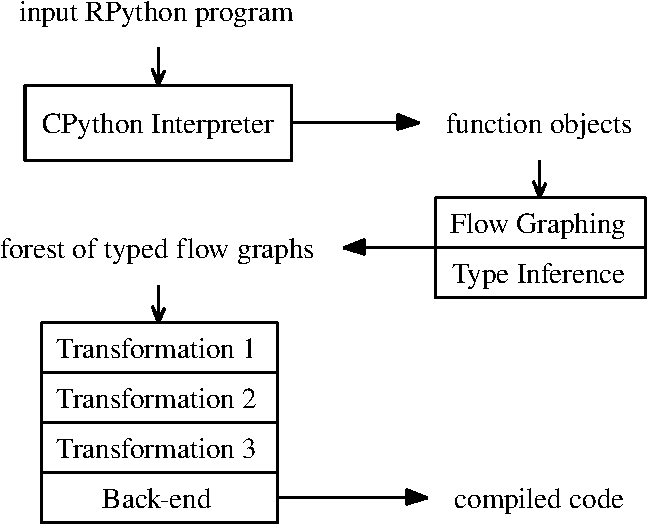
\includegraphics[width=5cm]{image/arch.pdf}
  \end{column}
  \begin{column}{7cm}
  \begin{itemize}
    \item
      Generate flow graphs from the RPython program
    \item
      Peform global type inference on the flow graphs
    \item
      Transform flow graphs through several steps until they match the level of
      the target environment
    \item
      Weave in translation aspects in the process
  \end{itemize}
  \end{column}
  \end{columns}

\end{frame}


\begin{frame}
  \frametitle{Translation Aspects (i)}
  Features not present in the source can be
  added during translation.

  Example: memory management:
  \begin{itemize}
  \item
  Boehm garbage collector
  \item
  mark-n-sweep written in RPython, with additional features
  \item
  reference counting
  \end{itemize}
\end{frame}


\begin{frame}
  \frametitle{Translation Aspects (ii)}
  \begin{itemize}
  \item
    \alert{Stackless transformation}: continuation capture, implemented by
    saving the low-level frames' local variables into the heap and back
    \begin{itemize}
      \item allows arbitrarily deep stack usage
      \item uses the C stack as long as possible
      \item has the consequence of making RPython do tail call elimination
    \end{itemize}
  \item
    work in progress: turning an interpreter into a just-in-time compiler
    is a translation aspect too
  \end{itemize}
\end{frame}

\section{The Prolog interpreter}
\begin{frame}
  \frametitle{Prolog Interpreter Implementation}
  \begin{itemize}
  \item
    naive, very simple interpreter
    \begin{itemize}
    \item uses "structure copying"
    \item interprets Prolog terms directly, no bytecode
    \end{itemize}
  \item
    uses continuation passing style similar to BinProlog
  \item
    Prolog calls mapped to RPython calls
    \begin{itemize}
    \item possible because stackless allows arbitrary deep recursion
    \end{itemize}
  \item
    implements large parts of the ISO standard (some builtins missing)
  \end{itemize}
\end{frame}




\begin{frame}
  \frametitle{Builtins}
  \begin{itemize}
  \item
    builtins implemented in Python
  \item
    easy to add new ones to interface with libraries
  \item
    application-specific builtins
  \item
    examples:
    \begin{itemize}
    \item functions to download and analyze webpages
    \item an imperative hashmap
    \end{itemize}
  \end{itemize}
\end{frame}


\begin{frame}
  \frametitle{Interpreter Facts}
  \begin{itemize}
  \item
    2500 lines of Python code in total
  \item
    700 of those are for builtins
  \item
    after translation to C: 14000 line of C code
  \item
    part of the PyPy distribution at:
    http://codespeak.net/pypy
  \end{itemize}
\end{frame}



\begin{frame}
  \frametitle{Performance (i)}
  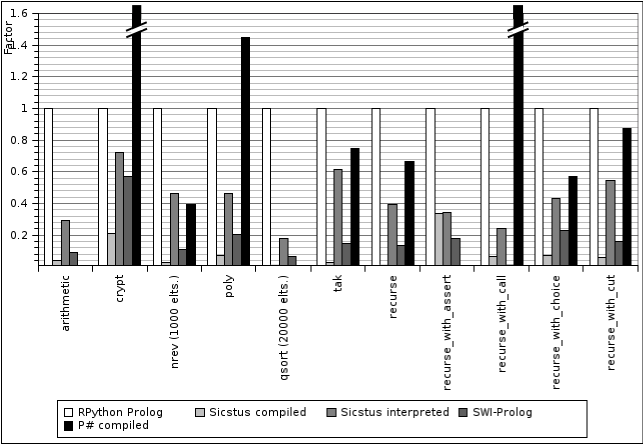
\includegraphics[scale=0.4]{image/bench.png}
\end{frame}


\begin{frame}
  \frametitle{Performance (ii)}
  \begin{itemize}
  \item
    performance is quite bad compared to tuned C implementations
  \item
    performance is pretty good compared to Java and .NET implementations
  \item
    surprising, since those are often based on the WAM
  \item
    maybe it's hard to simulate the WAM on such a VM
  \end{itemize}
\end{frame}

\begin{frame}
  \frametitle{Title}
  \begin{itemize}
  \item
  \end{itemize}
\end{frame}


\section*{Summary}
\subsection*{Summary}
\begin{frame}
  \frametitle<presentation>{Summary}

  % Keep the summary *very short*.
  \begin{itemize}
  \item
    The construction of virtual machines gets easier when using high-level
    languages
  \item
    XXX
  \item
    XXX
  \end{itemize}
\end{frame}
\subsection*{Outlook}
\begin{frame}
  \frametitle<presentation>{Outlook}
  % The following outlook is optional.
  \begin{itemize}
  \item
  \end{itemize}
\end{frame}



\end{document}


